\documentclass{article}
\usepackage{neurips_2026}
\usepackage[utf8]{inputenc}
\usepackage[T1]{fontenc}
\usepackage{hyperref}
\usepackage{url}
\usepackage{booktabs}
\usepackage{amsfonts,amsmath,amssymb,amsthm}
\usepackage{nicefrac}
\usepackage{microtype}
\usepackage{xcolor}
\usepackage{graphicx}
\graphicspath{{../figures/}}
\newtheorem{proposition}{Proposition}
\newcommand{\simplex}{\Delta^{K-1}}
\renewcommand{\Pr}{\mathbb{P}}
\DeclareMathOperator{\clr}{clr}

\title{Which Parts of Conformal Evaluation Survive on the Simplex? Validity, Efficiency and Conditional Coverage for Composition-Valued Predictions}

\author{Anonymous Author(s)}

\begin{document}
\maketitle

Predictions that are compositions, such as softmax vectors, topic proportions or vote distributions, can be given conformal regions on the simplex, but it is unclear how such methods should be evaluated and which scores suit which conditions. We study the evaluation of split conformal regions for composition-valued responses with seven scores (Euclidean, total variation, Hellinger, KL, Linf, Aitchison, Dirichlet likelihood), in plain, locally normalised and Mondrian variants, plus CV+. We verify that the finite-sample coverage law of split conformal prediction is score-free (a Beta law, checked for three scores and two noise families), so marginal coverage cannot discriminate between scores; we show that on class labels the total-variation, Hellinger and KL scores yield exactly the LAC label sets; and we calibrate binned conditional-coverage metrics against a null simulation in which conditional coverage is exact. In a synthetic grid of $48$ configurations with a known conditional law ($100$ replicates each), the ranking of scores by region mass depends on the noise law (the Aitchison region is $2.5$ times the Euclidean one for Dirichlet noise at $K=3$ but $0.9$ times for rounded logistic-normal noise at $K=10$), local normalisation repairs conditional coverage only under heteroscedasticity and never down to the null floor, Mondrian calibration by argmax is unusable at $30$ calibration points, and Aitchison region sizes change several-fold with the zero-replacement constant. A first-order Dirichlet theory predicts pointwise Euclidean conditional coverage (RMSE $\le0.010$) but fails for the Aitchison score. Experiments on CIFAR-10 and CIFAR-10H and a covariate-shift check complete a reproducible protocol; we claim no new guarantee and limit conclusions to the tested designs.

\section{Introduction}
Many predictors output a \emph{composition}: a non-negative vector that sums to one, such as a softmax probability vector, a vector of topic proportions or an annotator vote distribution. A user of such a prediction needs more than a point estimate; they need to know whether the attached uncertainty statement can be trusted. Split conformal prediction offers a finite-sample marginal coverage guarantee under exchangeability for any score function \citep{angelopoulos2021gentle}, and has been applied to label sets of classifiers \citep{angelopoulos2021raps,ding2023clustered}, to batch group-conditional guarantees \citep{jung2023batch} and, for composition-valued responses, to regions of the simplex \citep{javanmardi2024credal}. What is missing is an agreed, reproducible way to \emph{evaluate} such methods when the response lives on the simplex: the efficiency measure of a region of the simplex, the strata used to probe conditional coverage, the number of calibration points at which these diagnostics can be trusted, and which of the observed differences between scores are real.

We therefore treat evaluation itself as the object of study and ask: \emph{for composition-valued predictions, which parts of conformal evaluation are score-free guarantees, and which depend on the geometry of the score, the calibration scheme and the sample size?} We study a response $y\in\simplex$ and a regression $x\mapsto \hat p(x)\in\simplex$, and compare split-calibrated regions built from seven scores (Euclidean, total variation, Hellinger, KL, Aitchison/CLR, Linf and a Dirichlet negative log-likelihood), in plain, locally normalised and Mondrian variants, plus CV+. A synthetic oracle with a known conditional law provides ground truth for conditional coverage; CIFAR-10 softmax outputs and CIFAR-10H vote proportions give a real label-set bridge and a real composition-valued response.

\paragraph{Contributions.} (i) A concrete evaluation protocol for composition-valued conformal regions, with explicit choices of size measure, strata and uncertainty quantification (Section~\ref{sec:protocol}). (ii) An exact check, per score and family, of the finite-sample coverage law of split conformal prediction (Section~\ref{sec:theory}, Section~\ref{sec:exp}). (iii) An empirical comparison of scores and calibration schemes, with confidence intervals over repeated calibration sets and data seeds, and an oracle measurement of conditional coverage (Section~\ref{sec:exp}). (iv) A null simulation that quantifies how large a difference in binned conditional-coverage metrics must be to be interpretable at realistic sample sizes. (v) An explicit statement of where the conclusions hold and where they must not be extrapolated (Section~\ref{sec:disc}). We claim no new coverage guarantee and no conditional guarantee; our novelty claim is limited to the literature we read (Section~\ref{sec:related}).

\section{Related work}\label{sec:related}
\paragraph{Conformal prediction and its evaluation.} Split (inductive) conformal prediction calibrates a score threshold on held-out data; its coverage conditional on the calibration set follows a Beta law, and \citet{angelopoulos2021gentle} recommend comparing the empirical distribution of coverage over calibration draws with this law to separate implementation errors from fluctuation, and stress that adaptivity must be assessed separately from coverage. For classifiers, \citet{angelopoulos2021raps} introduce regularised adaptive sets and size-stratified coverage violation (SSCV), and \citet{ding2023clustered} evaluate class-conditional coverage gaps (CovGap) and set size over repeated splits when classes have few calibration points. \citet{jung2023batch} give group-conditional guarantees for any score and group collection; we do not run them (Section~\ref{sec:disc}). These works treat the softmax output as a score input and do not use the geometry of the simplex.

\paragraph{Multivariate and constrained responses.} \citet{feldman2023calibrated} calibrate multi-output quantile regions and compare region volume; \citet{principato2024hierarchical} show for responses satisfying linear equality constraints that projecting the point prediction onto the constraint set cannot increase an $A$-norm score, so regions shrink without losing coverage. Sum-to-one is such a constraint, but the simplex has additional inequality constraints $y\ge0$ that their equality-constraint result does not address.

\paragraph{Composition-valued responses.} The closest setting is \citet{javanmardi2024credal}, who conformalise credal sets: the response is an annotator label distribution and the output is a split-conformal region of the simplex defined through total variation, Wasserstein, KL, an inner-product score or a Dirichlet likelihood. Efficiency is measured as the fraction of a grid of the simplex covered (resolution $0.005$, $K=3$ in their main experiment), which does not scale to larger $K$. They report average coverage, but do not compare calibration schemes, probe conditional coverage, or use log-ratio geometry. We reuse the setting and the scores as a starting point and add the evaluation questions above.

\paragraph{Compositional data analysis.} \citet{aitchison1982statistical} models compositions through log-ratios; the Aitchison distance is the Euclidean distance between centred log-ratio (CLR) coordinates and requires strictly positive parts. Zeros, which occur whenever labels are one-hot or components fall below a detection limit, need a pre-declared replacement rule; we make that rule an experimental factor.

\section{Setting, methods and evaluation protocol}
\subsection{Setting and conformal regions}
Let $(X,Y)$ have $Y\in\simplex=\{y\in\mathbb{R}^K_{\ge0}:\sum_k y_k=1\}$, and let $\hat p:\mathcal X\to\simplex$ be a predictor trained on a fit split. Given a score $s(y,p)$ (larger = worse fit), a calibration set of size $n$ from a split independent of the fit split, and level $\alpha$, the split conformal threshold is $\hat q$, the $k$-th smallest calibration score with $k=\lceil (n+1)(1-\alpha)\rceil$ ($\hat q=\infty$ if $k>n$), and the region is $C(x)=\{y\in\simplex: s(y,\hat p(x))\le\hat q\}$.

\paragraph{Scores.} With $\tilde y=\mathrm{closure}(y+\varepsilon)$ for zero replacement: Euclidean $\|y-p\|_2$; total variation $\tfrac12\|y-p\|_1$; Hellinger $\|\sqrt y-\sqrt p\|_2$; $\mathrm{KL}(y\|p)$; $\|y-p\|_\infty$; Aitchison $\|\clr(\tilde y)-\clr(\tilde p)\|_2$; and the Dirichlet negative log-density $-\log \mathrm{Dir}(\tilde y;\hat\phi \tilde p)$ with a single precision $\hat\phi$ fitted by maximum likelihood on a separate split.

\paragraph{Calibration schemes.} \emph{Plain} split conformal; \emph{normalised} scores $s/\hat\sigma(x)$ where $\hat\sigma$ is a random forest for the score fitted on a third split; \emph{Mondrian} calibration with one threshold per predicted-dominant-part group; and \emph{CV+} with $10$ folds for the Euclidean score and a multinomial-logit predictor.

\subsection{Evaluation protocol}\label{sec:protocol}
\paragraph{Marginal validity.} For each configuration we repeat the whole pipeline (fresh data draw, fit, calibrate, test) $R$ times and report the mean test coverage with a confidence interval over replicates, and compare the empirical distribution of calibration-conditional coverage with the Beta law below.
\paragraph{Size.} A region's size is its Lebesgue measure on the simplex relative to the measure of the simplex, estimated by uniform Monte Carlo draws on $\simplex$ for $K\le5$ only; for larger $K$ the hit fraction vanishes and no volume is reported. Sizes under different reference measures (for example an Aitchison ball) are not compared with each other.
\paragraph{Conditional coverage.} Coverage is estimated within strata of the predicted maximal part and of the predicted entropy (quantile bins), within a boundary stratum ($\min_k y_k<0.01$), by worst-slab coverage \citep[a slab chosen on one half of the test data and evaluated on the other;][]{romano2020classification}, and, in the heteroscedastic worlds, by the true noise scale. On synthetic data these are measured against a known conditional law. We report the range of bin coverages (min/max), and calibrate their interpretability by a null simulation (Section~\ref{sec:exp}).

\subsection{Theory}\label{sec:theory}
\begin{proposition}[Coverage law of split conformal prediction]\label{prop:beta}
Let the calibration scores $S_1,\dots,S_n$ and the test score $S_{n+1}$ be exchangeable with continuous common distribution function $F$, independent of the fit split, and let $\hat q=S_{(k)}$ with $k=\lceil (n+1)(1-\alpha)\rceil\le n$. Then the coverage conditional on the calibration set, $V=\Pr(S_{n+1}\le\hat q\mid S_{1:n})=F(S_{(k)})$, has the law $\mathrm{Beta}(k,\,n+1-k)$. In particular $\mathbb E V=k/(n+1)\in[1-\alpha,\,1-\alpha+\tfrac1{n+1})$ and the law does not depend on $F$, hence not on the score, the predictor or the response family.
\end{proposition}
\begin{proof}
$F(S_i)$ are i.i.d.\ uniform by the probability integral transform, and the $k$-th order statistic of $n$ i.i.d.\ uniforms is $\mathrm{Beta}(k,n+1-k)$. The mean follows from $k\ge(n+1)(1-\alpha)$ and $k<(n+1)(1-\alpha)+1$.
\end{proof}
This is the finite-sample statement used to check the pipeline \citep{angelopoulos2021gentle}. It requires continuity of the score distribution: with exact zeros or rounded parts, ties can occur and $V$ stochastically dominates the Beta law (coverage $\ge1-\alpha$ but possibly conservative). Group-wise (Mondrian) calibration obeys the proposition within each group, with $n$ replaced by the random group size. Normalised scores stay valid because $\hat\sigma$ is fitted on a separate split. CV+ carries only a weaker guarantee ($\ge 1-2\alpha$ in general) and is not covered by the proposition.

\paragraph{Invariances.} Sets are unchanged under any strictly increasing transformation of the score (for instance Euclidean distance and its square), and the Aitchison ball is the same in every orthonormal ILR basis, since the Euclidean distance of CLR coordinates equals that of any orthonormal coordinates in the $(K-1)$-dimensional hyperplane. Only the \emph{shape} of the score matters for size and conditional coverage, not its monotone reparametrisation.


\begin{proposition}[Vertex labels]\label{prop:vertex}
If the response is a vertex $e_j$ (a class label), then total variation, Hellinger and $\mathrm{KL}(e_j\|p)$ are strictly decreasing functions of $p_j$ alone ($\tfrac12\|e_j-p\|_1=1-p_j$, $\|\sqrt{e_j}-\sqrt p\|_2^2=2-2\sqrt{p_j}$, $\mathrm{KL}=-\log p_j$), so the sets they induce coincide with those of the LAC score $1-p_j$. The Euclidean (Brier) score $\|e_j-p\|_2^2=1-2p_j+\|p\|_2^2$ and the Aitchison score depend on the rest of $p$, and generally give different sets.
\end{proposition}
This identifies which simplex scores are genuinely different from LAC on classifier outputs.

\paragraph{Pointwise conditional coverage under Dirichlet noise (large precision).} If $Y\mid x\sim\mathrm{Dir}(\phi\,\mu(x))$ and the predictor is $\mu(x)$, then for large $\phi$ the residual is approximately Gaussian with covariance $\Sigma_{\mathrm{L2}}=(\mathrm{diag}\,\mu-\mu\mu^\top)/(\phi+1)$ in raw coordinates, $\Sigma_{\mathrm{Ait}}=G\,\mathrm{diag}(\mu)^{-1}G/(\phi+1)$ in CLR coordinates ($G=I-\mathbf 1\mathbf 1^\top/K$), and $\Sigma_{\mathrm{Hel}}=(I-\sqrt\mu\sqrt\mu^\top)/(4(\phi+1))$ in Hellinger coordinates. Writing $\lambda_j(x)$ for the eigenvalues of $\Sigma(x)$, the squared score is approximately $\sum_j\lambda_j(x)Z_j^2$ with $Z_j$ i.i.d.\ standard normal; the marginal threshold $q$ is the $(1-\alpha)$ quantile of the $x$-mixture of these laws, and the predicted conditional coverage at $x$ is $\Pr(\sum_j\lambda_j(x)Z_j^2\le q^2)$. We check this first-order approximation by simulation in Section~\ref{sec:exp} and report where it fails; it is an approximation, not a theorem.

\section{Experiments}\label{sec:exp}
All numbers below are produced by the scripts listed in the reproduction notes (Appendix~\ref{app:repro}) from the committed result files; $\alpha=0.1$ is the primary level. A \emph{replicate} is an independent draw of data, predictor fit, calibration split and test set; intervals are $95\%$ $t$-intervals of the mean over replicates unless stated.

\subsection{Setup}
\paragraph{Synthetic worlds (E1).} $x\sim\mathcal N(0,I_4)$, mean $\mu(x)=\mathrm{softmax}(Bx+b)$ with a fixed random $(B,b)$ per configuration, $K\in\{3,5,10\}$. The conditional law is Dirichlet ($y\sim\mathrm{Dir}(\phi\mu)$, $\phi=20/h(x)$), logistic-normal ($y=\mathrm{softmax}(\log\mu+0.5\,h(x)\varepsilon)$), multinomial proportions ($30/h(x)$ counts, hence exact zeros) or a rounded logistic-normal with parts below $0.01$ set to zero. The noise factor is $h\equiv1$ (homoscedastic) or $h(x)=\exp(0.8\,w^\top x)$ (heteroscedastic). Predictors are a multinomial-logit regression on soft labels (the correct mean model for Dirichlet and multinomial noise, misspecified for the logistic-normal) and a random forest. Each replicate uses $1000$ points to fit, $500$ to fit $\hat\sigma$ and $\hat\phi$, $n$ calibration points (default $500$) and $2000$ test points.
\paragraph{Real data.} E2: a small CNN trained on CIFAR-10, with the test set split at random into calibration ($n=1000$) and test points, $200$ splits; label sets from the scores evaluated at the vertices. Two checkpoints (2 and 12 epochs; accuracy $0.740$ and $0.881$) vary the predictor's quality.

\subsection{Validity is score-free: the Beta law (C1)}
For each of three scores and two noise laws ($K=5$, linear predictor) we draw $3000$ calibration sets of size $n\in\{19,50,100,500\}$ and evaluate the calibration-conditional coverage on a test pool of $2\cdot10^6$ points. Fig.~\ref{fig:beta} shows the empirical mean and $5/95\%$ quantiles against the Beta band of Proposition~\ref{prop:beta}. The largest deviation of an empirical mean from the Beta mean over the $24$ cells is $0.002$; Kolmogorov--Smirnov $p$-values are $0.03$--$0.98$ (Dirichlet) and $0.02$--$0.86$ (multinomial), with $3$ of $24$ below $0.05$, consistent with chance given $24$ tests of which none is corrected. Note that this check uses the continuous noise laws; with exact zeros (E3, rounded worlds) ties only give the lower bound.
\begin{figure}[tbp]
\centering
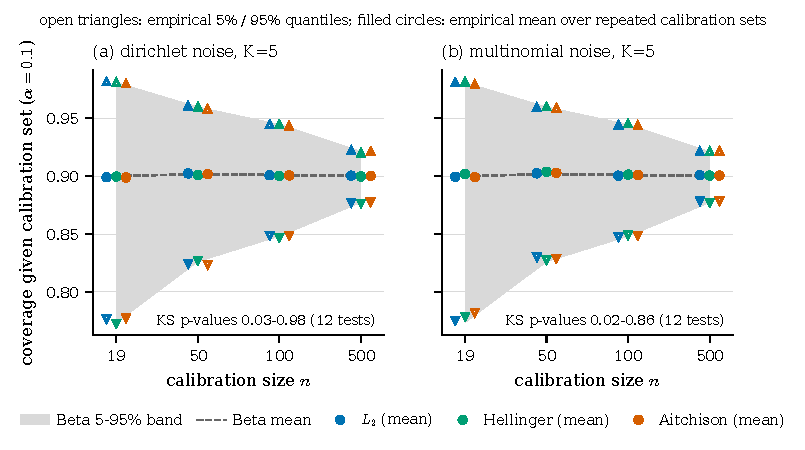
\includegraphics[width=0.85\linewidth]{fig1_beta_law.pdf}
\caption{Calibration-conditional coverage of split conformal prediction ($\alpha=0.1$, $K=5$, linear predictor) over $3000$ calibration sets per cell, for $L_2$, Hellinger and Aitchison scores. Shaded: exact $5$--$95\%$ band of $\mathrm{Beta}(k,n+1-k)$; markers: empirical mean and $5/95\%$ quantiles. KS $p$-values over the $12$ cells of each panel are annotated.}\label{fig:beta}
\end{figure}

\subsection{Efficiency of the regions depends on the score and on the noise law (C2)}
All $15$ main variants and CV+ are marginally valid in all $48$ configurations (mean coverage $0.896$--$0.909$), so differences in size compare equally valid regions. As efficiency measure we use the region \emph{mass} $\texttt{pool\_frac}$: the share of the marginal law of $y$ inside the region, estimated on the test pool. It is defined for every $K$, unlike the Lebesgue volume, which we compute only for $K\le5$ (Appendix, Fig.~\ref{fig:sizevol}; the Spearman correlation between mass and volume is $0.89$ at $K=3$ and $0.96$ at $K=5$). Fig.~\ref{fig:size} gives the mass relative to the plain $L_2$ region of the same replicate, for heteroscedastic worlds with a linear predictor.
\begin{figure}[tbp]
\centering
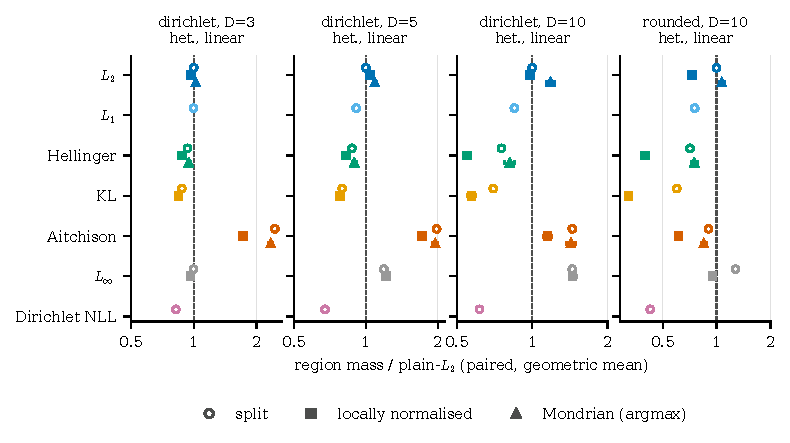
\includegraphics[width=0.85\linewidth]{fig2_size.pdf}
\caption{Region mass relative to the plain $L_2$ region of the same replicate (geometric mean over $100$ replicates; $95\%$ $t$-interval of the log ratio, mostly smaller than the markers), $\alpha=0.1$, $n_{\mathrm{cal}}=500$, heteroscedastic, linear predictor. Below $1$: more informative at equal coverage. Open: plain split; squares: locally normalised; triangles: Mondrian (argmax).}\label{fig:size}
\end{figure}
Three patterns stand out. (i) The ranking of scores is not stable across noise laws. The plain Aitchison region is $2.45$, $1.98$ and $1.45$ times the plain $L_2$ region for Dirichlet noise at $K=3,5,10$, but $0.90$ times for the rounded logistic-normal at $K=10$. (ii) The Dirichlet NLL score gives the smallest region in every Dirichlet panel ($0.82$, $0.67$, $0.62$ of $L_2$); the information-based scores follow (KL $0.88$, $0.80$, $0.70$; Hellinger $0.93$, $0.87$, $0.75$), whereas $L_\infty$ is no better than $L_2$ and worse for larger $K$ ($1.19$, $1.44$ at $K=5,10$). (iii) Local normalisation can shrink regions strongly at $K=10$ (normalised KL: $0.57$ of plain $L_2$ for Dirichlet noise and $0.32$ for the rounded world). Table~\ref{tab:e1} (Appendix~\ref{app:more}) gives all variants for $K=5$.

\subsection{Conditional coverage: normalisation helps under heteroscedasticity only (C3)}
Fig.~\ref{fig:cond} shows four conditional-coverage metrics at $K=5$, $n_{\mathrm{cal}}=500$, with the null band of Fig.~\ref{fig:null} in grey: the oracle gap $\overline{|c(x)-0.9|}$ from the known generator, the gap between the best and worst of five bins of the predicted top probability, worst-slab coverage, and coverage given $y$ near the boundary of the simplex (outcome-conditional and descriptive only).
\begin{figure}[tbp]
\centering
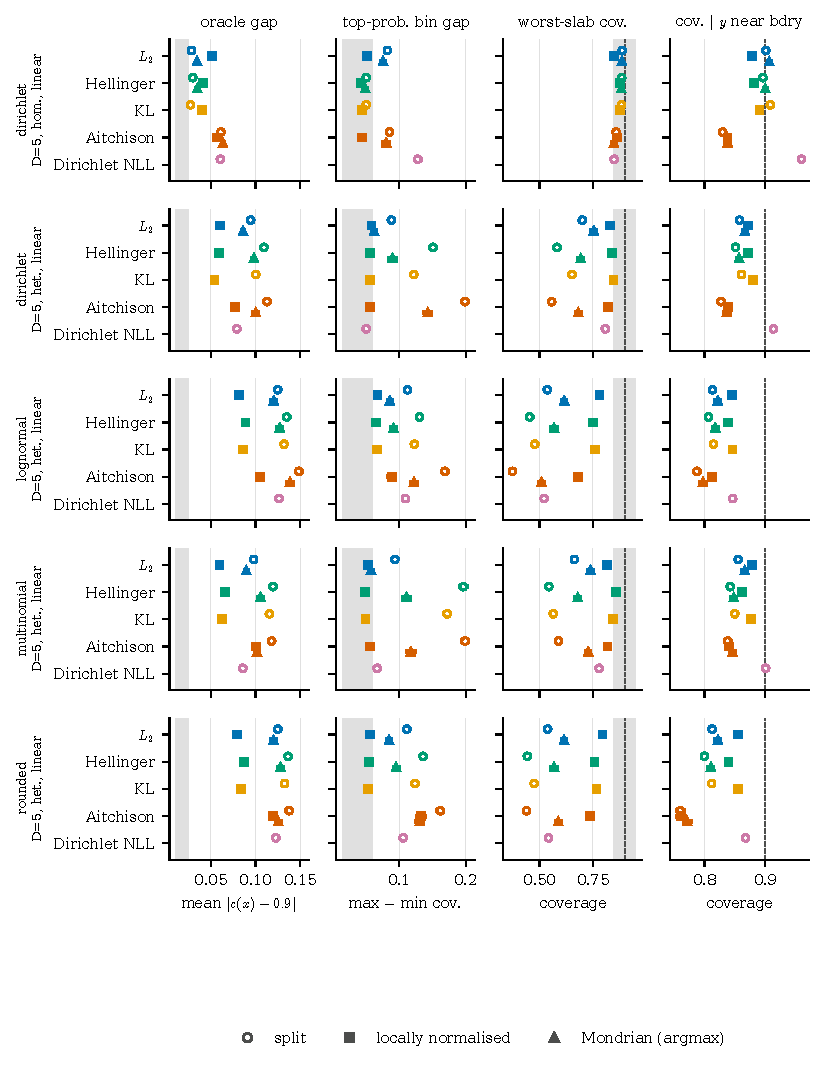
\includegraphics[width=\linewidth,height=0.42\textheight,keepaspectratio]{fig3_conditional.pdf}
\caption{Conditional-coverage metrics in five $K=5$ worlds ($n_{\mathrm{cal}}=500$, linear predictor, $100$ replicates; the $95\%$ intervals are smaller than the markers). Grey: $5$--$95\%$ band of the metric when conditional coverage is exact (Fig.~\ref{fig:null}); dashed: nominal $0.9$. Markers as in Fig.~\ref{fig:size}.}\label{fig:cond}
\end{figure}
Under homoscedastic Dirichlet noise the oracle gap of the $L_2$, $L_1$, $L_\infty$, Hellinger and KL scores is $0.026$--$0.030$, just above the null band ($0.011$--$0.025$), and local normalisation does not help (over the $24$ homoscedastic configurations the normalised score has the smaller gap in only $8$, with means $0.070$ against $0.062$). Under heteroscedastic noise every plain score is far from the null: the oracle gap is $0.079$--$0.148$ and worst-slab coverage as low as $0.37$--$0.60$, e.g. plain $L_2$ $0.118$ and $0.60$ against $0.083$ and $0.82$ for its normalised variant, which is better in all $24$ heteroscedastic configurations. Even the best variant (Dirichlet: normalised KL, gap $0.054$, wsc $0.85$; logistic-normal: normalised $L_\infty$, $0.077$, $0.81$) stays far above the floor, so normalisation by an estimated scale reduces but does not remove conditional miscoverage. The plain Aitchison score has the lowest worst-slab coverage in three of the four heteroscedastic rows ($0.56$ Dirichlet, $0.37$ logistic-normal, $0.44$ rounded; in the multinomial row Hellinger $0.54$ and Aitchison $0.59$ are lowest), and the plain Dirichlet NLL score is the best plain score only in its own world ($0.079$, wsc $0.81$; in the logistic-normal world its gap equals that of $L_2$, $0.126$ against $0.125$). Mondrian regions by argmax of the prediction improve plain scores less than scale normalisation (Table~\ref{tab:e1}). So no score is uniformly the best on both size and conditional coverage: the smallest mass is achieved by the Dirichlet NLL in its own world ($0.11$) but by normalised Aitchison ($0.21$, with a gap $0.105$) in the logistic-normal world.

\subsection{Calibration size and calibration scheme (C4)}
Fig.~\ref{fig:ncal} (Appendix~\ref{app:more}) varies $n_{\mathrm{cal}}\in\{30,100,250,500,2000\}$ ($K=5$, heteroscedastic, linear predictor). The standard deviation of test coverage over replicates follows $\sqrt{\mathrm{Var}\,\mathrm{Beta}(k,n+1-k)+0.09/2000}$, the Beta spread plus test-set noise, for all three scores shown, so the finite-sample coverage fluctuation is score-free also in this setting and shrinks from about $0.05$ to $0.01$. Region size behaves differently by scheme. Mondrian calibration by argmax needs enough points per group: at $n_{\mathrm{cal}}=30$ the threshold is infinite for $47\%$ of test points (the region is the whole simplex), coverage is $0.96$--$0.95$, and the median region volume is $0.73$ (Dirichlet) and $0.90$ (logistic-normal) against $0.13$ and $0.53$ for plain split; the difference is gone at $n_{\mathrm{cal}}=250$ in the Dirichlet world, and at $n_{\mathrm{cal}}=2000$ Mondrian is slightly smaller than plain split ($0.09$ against $0.11$; $0.38$ against $0.42$) but, for logistic-normal noise, not than the normalised variant. The locally normalised variant is stable in $n_{\mathrm{cal}}$ in these worlds; in the logistic-normal world it halves the region ($0.21$ against $0.53$ at $n_{\mathrm{cal}}=30$, $0.18$ against $0.42$ at $2000$). CV+ ($L_2$) has near-constant volume ($0.10$ and $0.42$) with coverage $0.90$ at every $n_{\mathrm{cal}}$; because it pools fitting and calibration data, its $n_{\mathrm{cal}}$ is not on the same footing as split conformal prediction, and CV+ was run for the linear predictor only.

\subsection{Zero replacement for the Aitchison score}
The Aitchison score needs parts replaced by $\varepsilon>0$. Marginal coverage is unaffected ($0.896$--$0.909$ for all plotted variants) but the region mass of the plain score falls from $0.52$--$0.63$ at $\varepsilon=10^{-4}$ to $0.13$--$0.31$ at $\varepsilon=0.1$ (Dirichlet $0.52\to0.14$, multinomial $0.57\to0.13$, rounded $0.63\to0.31$), while worst-slab coverage moves little and non-monotonically and stays below that of normalised $L_2$ (Fig.~\ref{fig:eps}, Appendix). The zero-replacement constant is therefore a tuning parameter of efficiency that must be reported; here the main grid used $\varepsilon=10^{-3}$.

\subsection{Label-set bridge on CIFAR-10 (C7)}
Table~\ref{tab:e2} gives results at $T=1$. All methods reach $0.900$ marginal coverage, as Proposition~\ref{prop:beta} implies. As Proposition~\ref{prop:vertex} states, $L_1$, Hellinger and KL sets are identical to LAC sets in $100\%$ of test points (column ``$=$LAC''), so these three are not different methods on classifier outputs; the Brier ($L_2$) and Aitchison sets differ from LAC in $2.8\%$ and $2$--$9\%$ of points at $12$ epochs. LAC has the smallest sets ($1.055$) but the largest class-conditional undercoverage (minimum per-class coverage $0.800$ against $0.872$ for APS at size $1.303$), which is the usual efficiency--adaptivity trade-off \citep{angelopoulos2021raps}. Which score is better on SSCV depends on the checkpoint and zero replacement: with $\varepsilon=10^{-3}$ the Aitchison score reaches SSCV$^\dagger$ $0.911$ at $12$ epochs but produces $2.6\%$ empty sets and a lower minimum class coverage ($0.794$), whereas $\varepsilon=0.1$ gives $0.814$; the Aitchison score on a softmax is thus sensitive to the zero-replacement constant.
\begin{table}[tbp]
\centering\small
\caption{CIFAR-10 label sets, $T=1$, $n_{\mathrm{cal}}=1000$, $200$ random calibration/test splits of the $10{,}000$ test images; mean $\pm$ half-width of the $95\%$ $t$-interval over splits. SSCV$^\dagger$: minimum coverage over size strata $\{1\},\{2\text{--}3\},\{4{+}\}$ (strata with fewer than $30$ points dropped). ``$=$LAC'': share of test points whose set equals the LAC set.}\label{tab:e2}
\resizebox{\linewidth}{!}{\input{../tables/tab3_e2_labelsets}}
\end{table}

\subsection{Conditional coverage under Dirichlet noise: where the first-order theory holds (C6)}
Fig.~\ref{fig:delta} (Appendix~\ref{app:more}) compares the delta-method prediction of Section~\ref{sec:theory} with simulated pointwise coverage (oracle mean predictor, $300$ values of $x$ per panel, precision $\phi\in\{200,50,20,8\}$). For the Euclidean score the prediction is accurate (RMSE $0.008$--$0.010$ across all four precisions; correlation $\ge0.94$). For the Hellinger score the first-order prediction is exactly flat at $0.9$ (the Gaussian approximation is variance-stabilised, which is why no correlation is defined), while the simulated coverage varies in $[0.81,0.99]$ with RMSE $0.014$--$0.038$ growing as $\phi$ falls; we only learn that Hellinger conditional coverage is much closer to homogeneous than Euclidean, not by how much. For the Aitchison score the approximation fails (RMSE $0.16$--$0.27$; correlation $0.58$ at $\phi=200$ falling to $-0.44$ at $\phi=8$, also for a second-order moment variant): we conjecture that the log-ratio score is dominated by the smallest parts, where the Gaussian approximation of a Dirichlet is poor, but we did not test this. We therefore claim the first-order prediction only for the Euclidean score in the tested range $\phi\ge8$, $K=5$.

\subsection{How large must a difference in conditional-coverage metrics be? (C5)}
Binned and worst-slab metrics are noisy and, being extrema over bins or slabs, biased even for a method with exact conditional coverage. We quantify this by a null simulation: for each $n_{\mathrm{cal}}$ we draw $500$ replicates in which the coverage level is $p\sim\mathrm{Beta}(k,n+1-k)$ (the exact split-conformal law) and coverage indicators on $2000$ test points are Bernoulli$(p)$ independent of the features, then apply the same binning and slab code as in E1 (Fig.~\ref{fig:null}). At $n_{\mathrm{cal}}=500$ the null gap between the highest and lowest of $5$ equal-mass bins of the predicted maximal part is $0.034$ (sd $0.013$), the null worst-slab coverage is $0.90$ (sd $0.03$), and the oracle pointwise gap (60 points, $400$ draws each) has a floor of $0.016$ (sd $0.005$) from Monte-Carlo noise and the calibration-induced deviation of $p$ from $0.9$. A difference between methods below these spreads is not interpretable, and we report conditional-coverage gaps in the following section only relative to this null band.
\begin{figure}[tbp]
\centering
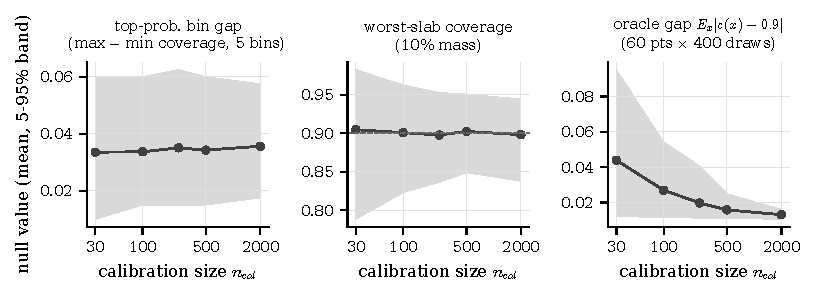
\includegraphics[width=0.85\linewidth]{fig5_null_spread.pdf}
\caption{Null distribution of three conditional-coverage metrics when conditional coverage is exact by construction ($n_{\mathrm{test}}=2000$, $500$ replicates per $n_{\mathrm{cal}}$). Line: mean; band: $5$--$95\%$.}\label{fig:null}
\end{figure}

\subsection{A real composition-valued response: CIFAR-10H (C8)}
CIFAR-10H gives, for each CIFAR-10 test image, the distribution of human labels, a composition with $80.6\%$ exact zeros; the predictor is the $12$-epoch CNN softmax ($T=1$). Because of the zeros and discrete vote proportions, scores tie and Proposition~\ref{prop:beta} guarantees only $\ge1-\alpha$; coverage refers to the noisy vote proportions, not to a latent label law. Dimension is $K=10$, so the Lebesgue volume is useless; as efficiency we use ``mass'', the share of the other images' human distributions that fall inside the region (lower is more informative at equal coverage). Table~\ref{tab:e3} (Appendix~\ref{app:more}; 100 random splits into $2000$/$1000$/rest for $\hat\sigma$, calibration and test) shows: (i) all $18$ variants reach marginal coverage $0.900$--$0.906$, slightly above $0.9$ for Mondrian ($0.905$--$0.906$), consistent with ties and small groups; (ii) plain and Mondrian regions have similar mass ($0.103$--$0.118$) for all scores, whereas locally normalised regions are $3$--$5$ times less informative ($0.32$--$0.56$) and do not repair conditional coverage; (iii) coverage in the worst of five confidence bins of the CNN stays at $0.63$--$0.75$ for every variant, far below $0.9$ and far outside the null band of Fig.~\ref{fig:null} (gap $0.034$); the entropy of the human distribution is an outcome-conditional diagnostic, not a conditioning variable of the guarantee, so its bin gaps need not vanish. We cannot rank scores on this dataset beyond this: the intervals of several rows overlap, and the single predictor, single dataset and tie structure limit what transfers.

\subsection{Covariate shift: a bounded check (C10)}
Section~\ref{sec:disc} excludes shift from the guarantees, but we check one family: $K=5$, heteroscedastic, linear predictor, calibration $x\sim\mathcal N(0,I)$ and test $x\sim\mathcal N(\delta w,I)$ with $w$ the direction of increasing noise, $n_{\mathrm{cal}}=500$, $100$ replicates. Fig.~\ref{fig:shift} (Appendix~\ref{app:more}) shows that ordinary split conformal prediction loses coverage as $\delta$ grows: at $\delta=1.5$ the plain scores fall to $0.49$--$0.73$ (logistic-normal $0.49$--$0.59$) and the locally normalised ones to $0.70$--$0.92$, so normalisation mitigates but does not remove the loss. Weighted split conformal prediction with the exact likelihood ratio \citep{tibshirani2019covariate} restores coverage to $0.895$--$0.920$ in all families and shifts, at the price of a smaller effective calibration size (down to $73$ at $\delta=1.5$). The exact likelihood ratio is known here; with estimated weights this is not guaranteed. This is one shift family on one predictor and supports no general statement about shift.

\section{Discussion and limitations}\label{sec:disc}
\paragraph{What is score-free and what is not.} The finite-sample marginal coverage law is score-free (Proposition~\ref{prop:beta}, Fig.~\ref{fig:beta}); it is the right first test of any evaluation pipeline, and it fails to discriminate between scores. Everything a user may care about beyond it, namely region size, coverage across the simplex and robustness to shift, depends on the score geometry, the noise law and the calibration scheme, and on classifier outputs several of the simplex scores collapse to the same sets (Proposition~\ref{prop:vertex}, Table~\ref{tab:e2}). Conditional-coverage metrics computed from bins or slabs have a null spread (Fig.~\ref{fig:null}) that must be reported next to any comparison.

\paragraph{Scope of the conclusions.} Results hold for exchangeable data; for the tested dimensions $K\in\{3,5,10\}$ and calibration sizes; for the generators described in Section~\ref{sec:exp} (fixed regression function per configuration, Gaussian covariates, two predictors); and for one CNN on CIFAR-10 and its CIFAR-10H annotations. They should not be extrapolated to (i) $K>10$ or to Lebesgue-volume comparisons for $K\ge 10$, where we use a different, dimension-valid measure (mass of a reference law) and compare scores only within it; (ii) full conformal or jackknife+ with neural predictors, which we did not run (CV+ is run only for the Euclidean score with the linear predictor); (iii) covariate or label shift beyond the single family in Section~\ref{sec:exp}; (iv) batch multivalid or other group-conditional methods \citep{jung2023batch}, which we did not run; (v) response distributions with heavy mass on the boundary other than those generated, in particular the zero-heavy CIFAR-10H proportions, where ties give only a lower bound.

\paragraph{Limitations.} We claim no new coverage guarantee and no conditional guarantee: exact conditional coverage is unattainable without assumptions, and the oracle measurements are specific to the generators. The delta-method prediction is first-order and fails for the Aitchison score at the tested precisions (Fig.~\ref{fig:delta}). The Aitchison and Dirichlet-likelihood scores depend on the zero-replacement constant $\varepsilon$, which we varied only in a sensitivity run. Efficiency depends on the reference measure (Lebesgue on the simplex, or the marginal law of $y$); rankings under the two may differ and we do not compare across them. RAPS is not tuned. Intervals reflect variability over data and calibration draws for fixed regression functions; they do not account for variation over the choice of regression function, since each configuration fixes one with seed $0$. The synthetic worlds were designed by us; their noise levels (e.g.\ $\phi_0=20$) determine how sharp the differences between scores are. Our novelty claim is limited to the literature we read (Section~\ref{sec:related}); we did not search exhaustively.


\bibliographystyle{plainnat}
\bibliography{refs}

\appendix
\section{Reproduction notes}\label{app:repro}
All code, result files and run commands are in the accompanying repository: \texttt{src/} (library), \texttt{scripts/} (experiment runners), \texttt{results/} (CSV files and a column guide), \texttt{figtab/} (one script per figure and table, with input files recorded in \texttt{figtab/MANIFEST.md}) and \texttt{REPRODUCE.md} (environment and package versions, data sources and versions, seeds, commands, expected run times, and the map from each exhibit to its script). Data: CIFAR-10 (copy from the Hugging Face dataset \texttt{uoft-cs/cifar10}, a fixed revision recorded in \texttt{REPRODUCE.md}; no licence stated by the source) and CIFAR-10H human label distributions (no licence stated); both are cited in \texttt{REPRODUCE.md}. No forbidden material was encountered; this is recorded there.


\paragraph{Exhibit map.} Numbering in the paper differs from the file names in \texttt{figures/} and \texttt{tables/}: Fig.~\ref{fig:beta} \texttt{fig1\_beta\_law}; Fig.~\ref{fig:size} \texttt{fig2\_size}; Fig.~\ref{fig:cond} \texttt{fig3\_conditional}; Fig.~\ref{fig:null} \texttt{fig5\_null\_spread}; Fig.~\ref{fig:ncal} \texttt{fig4\_ncal}; Fig.~\ref{fig:delta} \texttt{fig6\_delta\_method}; Fig.~\ref{fig:shift} \texttt{fig7\_shift}; Fig.~\ref{fig:sizevol} \texttt{fig2\_size\_volume}; Fig.~\ref{fig:eps} \texttt{fig8\_eps\_sensitivity}; Table~\ref{tab:e1} \texttt{tab2\_e1\_headline}; Table~\ref{tab:e2} \texttt{tab3\_e2\_labelsets}; Table~\ref{tab:e3} \texttt{tab4\_e3\_cifar10h}; Tables~\ref{tab:gridd}--\ref{tab:gridro} \texttt{tabA\_e1\_grid\_*}. Each is produced by the script of the same stem in \texttt{figtab/} from the result files named in \texttt{figtab/MANIFEST.md}.
\section{Additional E1 exhibits}\label{app:e1}
\begin{figure}[h]
\centering
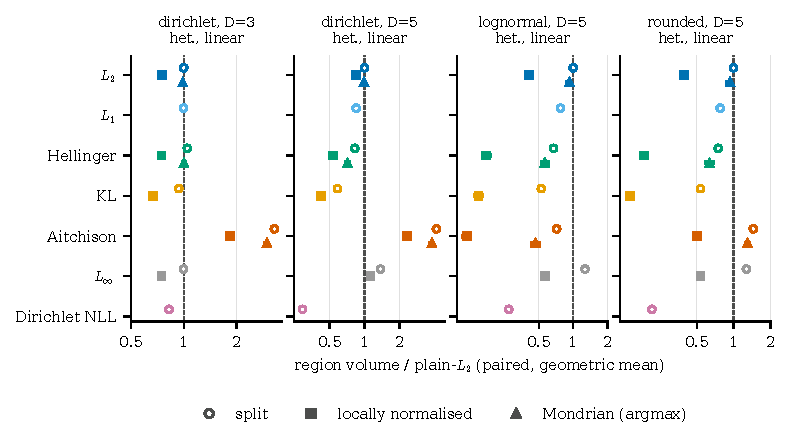
\includegraphics[width=\linewidth]{fig2_size_volume.pdf}
\caption{As Fig.~\ref{fig:size} with the Lebesgue volume of the region (Monte-Carlo) instead of the mass, in four configurations with $K\le5$ (Dirichlet $K=3,5$; logistic-normal and rounded $K=5$), where volume is computable.}\label{fig:sizevol}
\end{figure}
\begin{figure}[h]
\centering
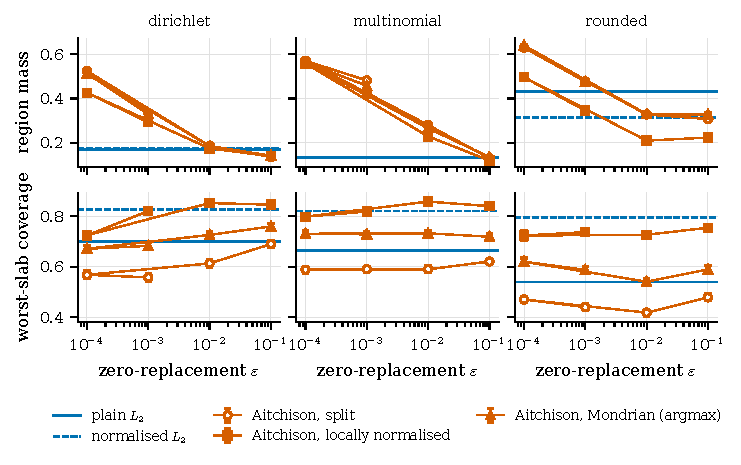
\includegraphics[width=\linewidth]{fig8_eps_sensitivity.pdf}
\caption{Sensitivity of the plain Aitchison score to the zero replacement $\varepsilon$ ($K=5$, heteroscedastic, linear predictor, $n_{\mathrm{cal}}=500$, $100$ replicates, $95\%$ $t$-intervals). Top: region mass; bottom: worst-slab coverage. Blue lines: plain and normalised $L_2$, independent of $\varepsilon$.}\label{fig:eps}
\end{figure}
\begin{table}[h]
\centering\scriptsize
\caption{All $12$ Dirichlet-noise configurations of the E1 grid ($n_{\mathrm{cal}}=500$, $100$ replicates; means; largest $95\%$ half-widths: oracle gap $0.004$, wsc $0.015$, mass $0.01$). cov.\ range: minimum--maximum over the $16$ methods of mean coverage. Oracle gap and wsc for plain and normalised $L_2$; mass for plain $L_2$, KL, Aitchison and Dirichlet NLL. Logistic-normal, multinomial and rounded: Tables~\ref{tab:gridln}--\ref{tab:gridro}.}\label{tab:gridd}
\input{../tables/tabA_e1_grid_dirichlet}
\end{table}
\begin{table}[h]
\centering\scriptsize
\caption{As Table~\ref{tab:gridd}, logistic-normal noise.}\label{tab:gridln}
\input{../tables/tabA_e1_grid_lognormal}
\end{table}
\begin{table}[h]
\centering\scriptsize
\caption{As Table~\ref{tab:gridd}, multinomial noise.}\label{tab:gridmn}
\input{../tables/tabA_e1_grid_multinomial}
\end{table}
\begin{table}[h]
\centering\scriptsize
\caption{As Table~\ref{tab:gridd}, rounded logistic-normal noise.}\label{tab:gridro}
\input{../tables/tabA_e1_grid_rounded}
\end{table}

\section{Further exhibits for Section~\ref{sec:exp}}\label{app:more}
\begin{figure}[h]
\centering
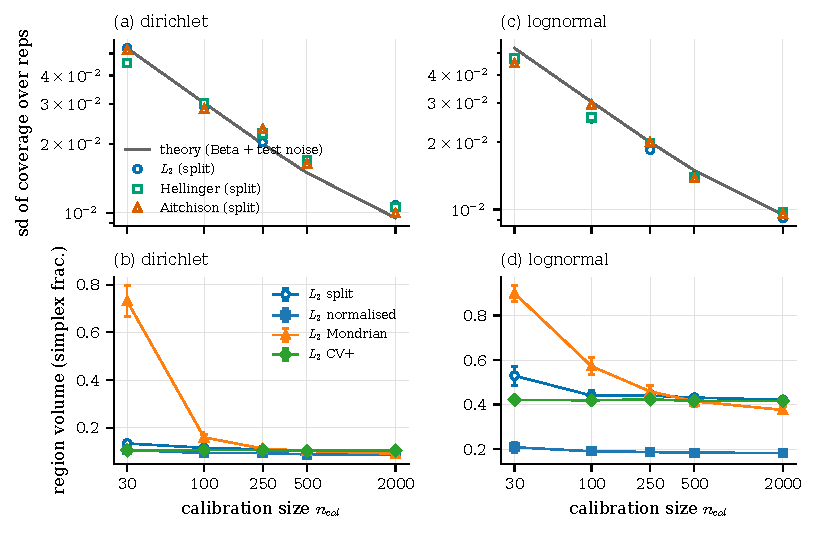
\includegraphics[width=\linewidth]{fig4_ncal.pdf}
\caption{Calibration size ($K=5$, heteroscedastic, linear predictor, $100$ replicates per point). (a,c) Standard deviation over replicates of test coverage; line: $\sqrt{\mathrm{Var}\,\mathrm{Beta}+0.09/2000}$. (b,d) Median region volume (fraction of the simplex) with $95\%$ $t$-intervals for split, locally normalised and Mondrian $L_2$ and for CV+; $n_{\mathrm{cal}}=500$ points come from the main grid.}\label{fig:ncal}
\end{figure}
\begin{figure}[h]
\centering
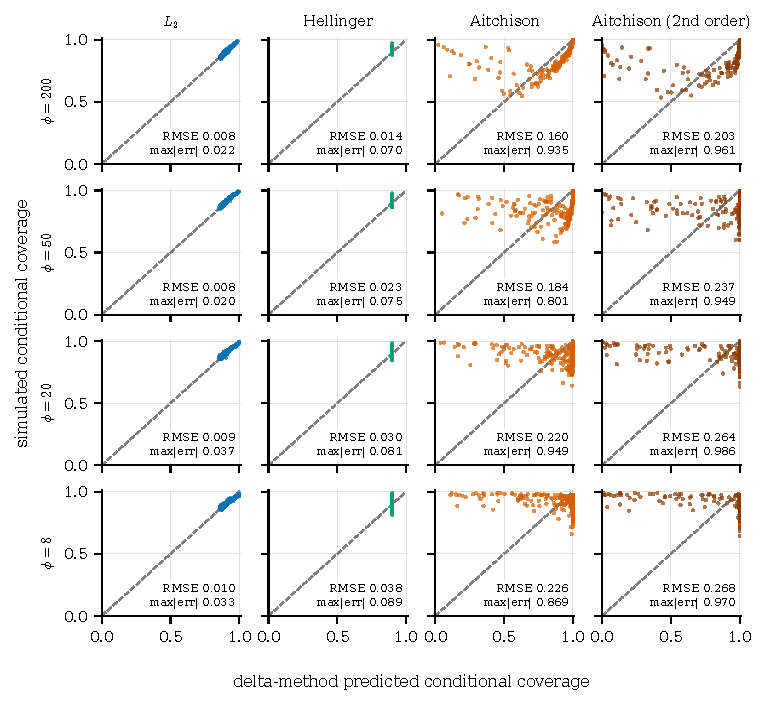
\includegraphics[width=\linewidth]{fig6_delta_method.pdf}
\caption{Delta-method prediction (horizontal) against simulated pointwise conditional coverage (vertical) of the marginal threshold at nominal $0.9$, $K=5$, Dirichlet noise, oracle mean predictor. Rows: precision $\phi$; columns: score (Aitchison in first-order and second-order moment versions). Dashed: identity.}\label{fig:delta}
\end{figure}
\begin{table}[h]
\centering\small
\caption{CIFAR-10H as a composition-valued response, $12$-epoch CNN softmax, $\alpha=0.1$, $n_{\mathrm{cal}}=1000$, $100$ random splits; mean $\pm$ half-width of the $95\%$ $t$-interval. mass: share of $300$ other images' human distributions inside the region; ambig.\ min / conf.\ min: coverage in the worst of $5$ equal-mass bins of the entropy of the human distribution / of the CNN's top-1 probability; wsc: worst-slab coverage ($\delta=0.1$).}\label{tab:e3}
\resizebox{\linewidth}{!}{\input{../tables/tab4_e3_cifar10h}}
\end{table}
\begin{figure}[h]
\centering
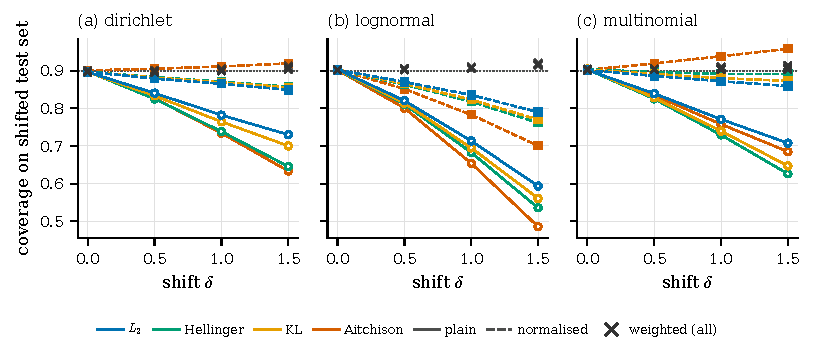
\includegraphics[width=\linewidth]{fig7_shift.pdf}
\caption{Test coverage under covariate shift of size $\delta$ towards noisier inputs ($K=5$, heteroscedastic, linear predictor, $n_{\mathrm{cal}}=500$, $100$ replicates). Lines: ordinary split conformal (solid: plain, dashed: locally normalised) with $95\%$ $t$-intervals; crosses: weighted split conformal with the exact likelihood ratio.}\label{fig:shift}
\end{figure}
\begin{table}[h]
\centering\small
\caption{E1, $K=5$, heteroscedastic, linear predictor, $n_{\mathrm{cal}}=500$, means over $100$ replicates (largest $95\%$ half-widths: coverage $0.004$, wsc $0.016$, oracle gap $0.004$, mass $0.009$). wsc: worst-slab coverage; or.\ gap: oracle conditional-coverage gap (null floor $0.011$--$0.025$); mass: region mass. Bold: best of the $15$ methods in the column (no significance claim).}\label{tab:e1}
\input{../tables/tab2_e1_headline}
\end{table}


\clearpage
\section*{NeurIPS Paper Checklist}

\begin{enumerate}

\item {\bf Claims}
    \item[] Question: Do the main claims made in the abstract and introduction accurately reflect the paper's contributions and scope?
    \item[] Answer: \answerYes{} % Replace by \answerYes{}, \answerNo{}, or \answerNA{}.
    \item[] Justification: The abstract and introduction state the scope (composition-valued responses, tested generators, one CNN) and claim no new guarantee; results are in Sec.~\ref{sec:exp}, limits in Sec.~\ref{sec:disc}.
    \item[] Guidelines:
    \begin{itemize}
        \item The answer \answerNA{} means that the abstract and introduction do not include the claims made in the paper.
        \item The abstract and/or introduction should clearly state the claims made, including the contributions made in the paper and important assumptions and limitations. A \answerNo{} or \answerNA{} answer to this question will not be perceived well by the reviewers. 
        \item The claims made should match theoretical and experimental results, and reflect how much the results can be expected to generalize to other settings. 
        \item It is fine to include aspirational goals as motivation as long as it is clear that these goals are not attained by the paper. 
    \end{itemize}

\item {\bf Limitations}
    \item[] Question: Does the paper discuss the limitations of the work performed by the authors?
    \item[] Answer: \answerYes{} % Replace by \answerYes{}, \answerNo{}, or \answerNA{}.
    \item[] Justification: Sec.~\ref{sec:disc} lists the limitations: exchangeability, tested $K\le10$, generators and predictors, one CNN and dataset, failure of the delta method for the Aitchison score, dependence on the zero replacement.
    \item[] Guidelines:
    \begin{itemize}
        \item The answer \answerNA{} means that the paper has no limitation while the answer \answerNo{} means that the paper has limitations, but those are not discussed in the paper. 
        \item The authors are encouraged to create a separate ``Limitations'' section in their paper.
        \item The paper should point out any strong assumptions and how robust the results are to violations of these assumptions (e.g., independence assumptions, noiseless settings, model well-specification, asymptotic approximations only holding locally). The authors should reflect on how these assumptions might be violated in practice and what the implications would be.
        \item The authors should reflect on the scope of the claims made, e.g., if the approach was only tested on a few datasets or with a few runs. In general, empirical results often depend on implicit assumptions, which should be articulated.
        \item The authors should reflect on the factors that influence the performance of the approach. For example, a facial recognition algorithm may perform poorly when image resolution is low or images are taken in low lighting. Or a speech-to-text system might not be used reliably to provide closed captions for online lectures because it fails to handle technical jargon.
        \item The authors should discuss the computational efficiency of the proposed algorithms and how they scale with dataset size.
        \item If applicable, the authors should discuss possible limitations of their approach to address problems of privacy and fairness.
        \item While the authors might fear that complete honesty about limitations might be used by reviewers as grounds for rejection, a worse outcome might be that reviewers discover limitations that aren't acknowledged in the paper. The authors should use their best judgment and recognize that individual actions in favor of transparency play an important role in developing norms that preserve the integrity of the community. Reviewers will be specifically instructed to not penalize honesty concerning limitations.
    \end{itemize}

\item {\bf Theory assumptions and proofs}
    \item[] Question: For each theoretical result, does the paper provide the full set of assumptions and a complete (and correct) proof?
    \item[] Answer: \answerYes{} % Replace by \answerYes{}, \answerNo{}, or \answerNA{}.
    \item[] Justification: Propositions~\ref{prop:beta} and~\ref{prop:vertex} state their assumptions (exchangeability; continuous scores for equality, ties give a lower bound) and are proved in Sec.~\ref{sec:theory}; the delta-method result is a stated first-order approximation, not a theorem.
    \item[] Guidelines:
    \begin{itemize}
        \item The answer \answerNA{} means that the paper does not include theoretical results. 
        \item All the theorems, formulas, and proofs in the paper should be numbered and cross-referenced.
        \item All assumptions should be clearly stated or referenced in the statement of any theorems.
        \item The proofs can either appear in the main paper or the supplemental material, but if they appear in the supplemental material, the authors are encouraged to provide a short proof sketch to provide intuition. 
        \item Inversely, any informal proof provided in the core of the paper should be complemented by formal proofs provided in appendix or supplemental material.
        \item Theorems and Lemmas that the proof relies upon should be properly referenced. 
    \end{itemize}

    \item {\bf Experimental result reproducibility}
    \item[] Question: Does the paper fully disclose all the information needed to reproduce the main experimental results of the paper to the extent that it affects the main claims and/or conclusions of the paper (regardless of whether the code and data are provided or not)?
    \item[] Answer: \answerYes{} % Replace by \answerYes{}, \answerNo{}, or \answerNA{}.
    \item[] Justification: Sec.~\ref{sec:exp} (setup), Sec.~\ref{sec:protocol} and Appendix~\ref{app:repro} give generators, predictors, splits, sizes, replicates and seeds; \texttt{REPRODUCE.md} lists package versions and commands.
    \item[] Guidelines:
    \begin{itemize}
        \item The answer \answerNA{} means that the paper does not include experiments.
        \item If the paper includes experiments, a \answerNo{} answer to this question will not be perceived well by the reviewers: Making the paper reproducible is important, regardless of whether the code and data are provided or not.
        \item If the contribution is a dataset and\slash or model, the authors should describe the steps taken to make their results reproducible or verifiable. 
        \item Depending on the contribution, reproducibility can be accomplished in various ways. For example, if the contribution is a novel architecture, describing the architecture fully might suffice, or if the contribution is a specific model and empirical evaluation, it may be necessary to either make it possible for others to replicate the model with the same dataset, or provide access to the model. In general. releasing code and data is often one good way to accomplish this, but reproducibility can also be provided via detailed instructions for how to replicate the results, access to a hosted model (e.g., in the case of a large language model), releasing of a model checkpoint, or other means that are appropriate to the research performed.
        \item While NeurIPS does not require releasing code, the conference does require all submissions to provide some reasonable avenue for reproducibility, which may depend on the nature of the contribution. For example
        \begin{enumerate}
            \item If the contribution is primarily a new algorithm, the paper should make it clear how to reproduce that algorithm.
            \item If the contribution is primarily a new model architecture, the paper should describe the architecture clearly and fully.
            \item If the contribution is a new model (e.g., a large language model), then there should either be a way to access this model for reproducing the results or a way to reproduce the model (e.g., with an open-source dataset or instructions for how to construct the dataset).
            \item We recognize that reproducibility may be tricky in some cases, in which case authors are welcome to describe the particular way they provide for reproducibility. In the case of closed-source models, it may be that access to the model is limited in some way (e.g., to registered users), but it should be possible for other researchers to have some path to reproducing or verifying the results.
        \end{enumerate}
    \end{itemize}


\item {\bf Open access to data and code}
    \item[] Question: Does the paper provide open access to the data and code, with sufficient instructions to faithfully reproduce the main experimental results, as described in supplemental material?
    \item[] Answer: \answerYes{} % Replace by \answerYes{}, \answerNo{}, or \answerNA{}.
    \item[] Justification: Code, result CSV files and per-exhibit generator scripts are in the delivered repository; data sources (Hugging Face CIFAR-10 copy, CIFAR-10H) and exact commands are in \texttt{REPRODUCE.md} (Appendix~\ref{app:repro}).
    \item[] Guidelines:
    \begin{itemize}
        \item The answer \answerNA{} means that paper does not include experiments requiring code.
        \item Please see the NeurIPS code and data submission guidelines (\url{https://neurips.cc/public/guides/CodeSubmissionPolicy}) for more details.
        \item While we encourage the release of code and data, we understand that this might not be possible, so \answerNo{} is an acceptable answer. Papers cannot be rejected simply for not including code, unless this is central to the contribution (e.g., for a new open-source benchmark).
        \item The instructions should contain the exact command and environment needed to run to reproduce the results. See the NeurIPS code and data submission guidelines (\url{https://neurips.cc/public/guides/CodeSubmissionPolicy}) for more details.
        \item The authors should provide instructions on data access and preparation, including how to access the raw data, preprocessed data, intermediate data, and generated data, etc.
        \item The authors should provide scripts to reproduce all experimental results for the new proposed method and baselines. If only a subset of experiments are reproducible, they should state which ones are omitted from the script and why.
        \item At submission time, to preserve anonymity, the authors should release anonymized versions (if applicable).
        \item Providing as much information as possible in supplemental material (appended to the paper) is recommended, but including URLs to data and code is permitted.
    \end{itemize}


\item {\bf Experimental setting/details}
    \item[] Question: Does the paper specify all the training and test details (e.g., data splits, hyperparameters, how they were chosen, type of optimizer) necessary to understand the results?
    \item[] Answer: \answerYes{} % Replace by \answerYes{}, \answerNo{}, or \answerNA{}.
    \item[] Justification: Data generators, splits, the CNN (epochs, accuracy), random-forest scale model, precision fit and the zero-replacement constants are given in Sec.~\ref{sec:exp} and in \texttt{REPRODUCE.md}; hyperparameters were fixed in advance and not tuned on test results (RAPS was not tuned).
    \item[] Guidelines:
    \begin{itemize}
        \item The answer \answerNA{} means that the paper does not include experiments.
        \item The experimental setting should be presented in the core of the paper to a level of detail that is necessary to appreciate the results and make sense of them.
        \item The full details can be provided either with the code, in appendix, or as supplemental material.
    \end{itemize}

\item {\bf Experiment statistical significance}
    \item[] Question: Does the paper report error bars suitably and correctly defined or other appropriate information about the statistical significance of the experiments?
    \item[] Answer: \answerYes{} % Replace by \answerYes{}, \answerNo{}, or \answerNA{}.
    \item[] Justification: Intervals are $95\%$ $t$-intervals over replicates (stated in captions); a null simulation quantifies the spread of the conditional-coverage metrics (Sec.~\ref{sec:exp}); Table~\ref{tab:e1} and tables in the appendix report means with the largest half-width.
    \item[] Guidelines:
    \begin{itemize}
        \item The answer \answerNA{} means that the paper does not include experiments.
        \item The authors should answer \answerYes{} if the results are accompanied by error bars, confidence intervals, or statistical significance tests, at least for the experiments that support the main claims of the paper.
        \item The factors of variability that the error bars are capturing should be clearly stated (for example, train/test split, initialization, random drawing of some parameter, or overall run with given experimental conditions).
        \item The method for calculating the error bars should be explained (closed form formula, call to a library function, bootstrap, etc.)
        \item The assumptions made should be given (e.g., Normally distributed errors).
        \item It should be clear whether the error bar is the standard deviation or the standard error of the mean.
        \item It is OK to report 1-sigma error bars, but one should state it. The authors should preferably report a 2-sigma error bar than state that they have a 96\% CI, if the hypothesis of Normality of errors is not verified.
        \item For asymmetric distributions, the authors should be careful not to show in tables or figures symmetric error bars that would yield results that are out of range (e.g., negative error rates).
        \item If error bars are reported in tables or plots, the authors should explain in the text how they were calculated and reference the corresponding figures or tables in the text.
    \end{itemize}

\item {\bf Experiments compute resources}
    \item[] Question: For each experiment, does the paper provide sufficient information on the computer resources (type of compute workers, memory, time of execution) needed to reproduce the experiments?
    \item[] Answer: \answerYes{} % Replace by \answerYes{}, \answerNo{}, or \answerNA{}.
    \item[] Justification: Appendix~\ref{app:repro} and \texttt{REPRODUCE.md} give the hardware (2 CPUs, 4~GB, no GPU) and expected run time of each step, e.g.\ about $25$ min for the CNN and $1.5$--$3$ h for the E1 grid.
    \item[] Guidelines:
    \begin{itemize}
        \item The answer \answerNA{} means that the paper does not include experiments.
        \item The paper should indicate the type of compute workers CPU or GPU, internal cluster, or cloud provider, including relevant memory and storage.
        \item The paper should provide the amount of compute required for each of the individual experimental runs as well as estimate the total compute. 
        \item The paper should disclose whether the full research project required more compute than the experiments reported in the paper (e.g., preliminary or failed experiments that didn't make it into the paper). 
    \end{itemize}
    
\item {\bf Code of ethics}
    \item[] Question: Does the research conducted in the paper conform, in every respect, with the NeurIPS Code of Ethics \url{https://neurips.cc/public/EthicsGuidelines}?
    \item[] Answer: \answerYes{} % Replace by \answerYes{}, \answerNo{}, or \answerNA{}.
    \item[] Justification: The work uses public data, simulation and standard models, involves no new human-subject data and no sensitive attributes, and follows the Code of Ethics.
    \item[] Guidelines:
    \begin{itemize}
        \item The answer \answerNA{} means that the authors have not reviewed the NeurIPS Code of Ethics.
        \item If the authors answer \answerNo, they should explain the special circumstances that require a deviation from the Code of Ethics.
        \item The authors should make sure to preserve anonymity (e.g., if there is a special consideration due to laws or regulations in their jurisdiction).
    \end{itemize}


\item {\bf Broader impacts}
    \item[] Question: Does the paper discuss both potential positive societal impacts and negative societal impacts of the work performed?
    \item[] Answer: \answerNA{} % Replace by \answerYes{}, \answerNo{}, or \answerNA{}.
    \item[] Justification: The paper is methodological with a simulation and public-dataset evaluation and has no direct societal application; the only consequence is that conformal uncertainty statements on compositions should be interpreted with the limits stated in Sec.~\ref{sec:disc}.
    \item[] Guidelines:
    \begin{itemize}
        \item The answer \answerNA{} means that there is no societal impact of the work performed.
        \item If the authors answer \answerNA{} or \answerNo, they should explain why their work has no societal impact or why the paper does not address societal impact.
        \item Examples of negative societal impacts include potential malicious or unintended uses (e.g., disinformation, generating fake profiles, surveillance), fairness considerations (e.g., deployment of technologies that could make decisions that unfairly impact specific groups), privacy considerations, and security considerations.
        \item The conference expects that many papers will be foundational research and not tied to particular applications, let alone deployments. However, if there is a direct path to any negative applications, the authors should point it out. For example, it is legitimate to point out that an improvement in the quality of generative models could be used to generate Deepfakes for disinformation. On the other hand, it is not needed to point out that a generic algorithm for optimizing neural networks could enable people to train models that generate Deepfakes faster.
        \item The authors should consider possible harms that could arise when the technology is being used as intended and functioning correctly, harms that could arise when the technology is being used as intended but gives incorrect results, and harms following from (intentional or unintentional) misuse of the technology.
        \item If there are negative societal impacts, the authors could also discuss possible mitigation strategies (e.g., gated release of models, providing defenses in addition to attacks, mechanisms for monitoring misuse, mechanisms to monitor how a system learns from feedback over time, improving the efficiency and accessibility of ML).
    \end{itemize}
    
\item {\bf Safeguards}
    \item[] Question: Does the paper describe safeguards that have been put in place for responsible release of data or models that have a high risk for misuse (e.g., pre-trained language models, image generators, or scraped datasets)?
    \item[] Answer: \answerNA{} % Replace by \answerYes{}, \answerNo{}, or \answerNA{}.
    \item[] Justification: No pre-trained generative model, scraped dataset or other high-risk asset is released; the small CIFAR-10 CNN poses no misuse risk.
    \item[] Guidelines:
    \begin{itemize}
        \item The answer \answerNA{} means that the paper poses no such risks.
        \item Released models that have a high risk for misuse or dual-use should be released with necessary safeguards to allow for controlled use of the model, for example by requiring that users adhere to usage guidelines or restrictions to access the model or implementing safety filters. 
        \item Datasets that have been scraped from the Internet could pose safety risks. The authors should describe how they avoided releasing unsafe images.
        \item We recognize that providing effective safeguards is challenging, and many papers do not require this, but we encourage authors to take this into account and make a best faith effort.
    \end{itemize}

\item {\bf Licenses for existing assets}
    \item[] Question: Are the creators or original owners of assets (e.g., code, data, models), used in the paper, properly credited and are the license and terms of use explicitly mentioned and properly respected?
    \item[] Answer: \answerYes{} % Replace by \answerYes{}, \answerNo{}, or \answerNA{}.
    \item[] Justification: CIFAR-10 (Krizhevsky, 2009, accessed via the Hugging Face copy) and CIFAR-10H (Peterson et al., 2019) are credited in \texttt{REPRODUCE.md}; the sources state no licence, which is recorded there, and use is for research only.
    \item[] Guidelines:
    \begin{itemize}
        \item The answer \answerNA{} means that the paper does not use existing assets.
        \item The authors should cite the original paper that produced the code package or dataset.
        \item The authors should state which version of the asset is used and, if possible, include a URL.
        \item The name of the license (e.g., CC-BY 4.0) should be included for each asset.
        \item For scraped data from a particular source (e.g., website), the copyright and terms of service of that source should be provided.
        \item If assets are released, the license, copyright information, and terms of use in the package should be provided. For popular datasets, \url{paperswithcode.com/datasets} has curated licenses for some datasets. Their licensing guide can help determine the license of a dataset.
        \item For existing datasets that are re-packaged, both the original license and the license of the derived asset (if it has changed) should be provided.
        \item If this information is not available online, the authors are encouraged to reach out to the asset's creators.
    \end{itemize}

\item {\bf New assets}
    \item[] Question: Are new assets introduced in the paper well documented and is the documentation provided alongside the assets?
    \item[] Answer: \answerYes{} % Replace by \answerYes{}, \answerNo{}, or \answerNA{}.
    \item[] Justification: The delivered code and result files are documented by \texttt{REPRODUCE.md} and \texttt{results/README.md} (column guide, exhibit-to-script map); no new dataset is released beyond simulated results.
    \item[] Guidelines:
    \begin{itemize}
        \item The answer \answerNA{} means that the paper does not release new assets.
        \item Researchers should communicate the details of the dataset\slash code\slash model as part of their submissions via structured templates. This includes details about training, license, limitations, etc. 
        \item The paper should discuss whether and how consent was obtained from people whose asset is used.
        \item At submission time, remember to anonymize your assets (if applicable). You can either create an anonymized URL or include an anonymized zip file.
    \end{itemize}

\item {\bf Crowdsourcing and research with human subjects}
    \item[] Question: For crowdsourcing experiments and research with human subjects, does the paper include the full text of instructions given to participants and screenshots, if applicable, as well as details about compensation (if any)? 
    \item[] Answer: \answerNA{} % Replace by \answerYes{}, \answerNo{}, or \answerNA{}.
    \item[] Justification: No crowdsourcing or new human-subject research was performed; CIFAR-10H annotations are an existing public dataset used as a response.
    \item[] Guidelines:
    \begin{itemize}
        \item The answer \answerNA{} means that the paper does not involve crowdsourcing nor research with human subjects.
        \item Including this information in the supplemental material is fine, but if the main contribution of the paper involves human subjects, then as much detail as possible should be included in the main paper. 
        \item According to the NeurIPS Code of Ethics, workers involved in data collection, curation, or other labor should be paid at least the minimum wage in the country of the data collector. 
    \end{itemize}

\item {\bf Institutional review board (IRB) approvals or equivalent for research with human subjects}
    \item[] Question: Does the paper describe potential risks incurred by study participants, whether such risks were disclosed to the subjects, and whether Institutional Review Board (IRB) approvals (or an equivalent approval/review based on the requirements of your country or institution) were obtained?
    \item[] Answer: \answerNA{} % Replace by \answerYes{}, \answerNo{}, or \answerNA{}.
    \item[] Justification: No new human-subject research was performed, so no IRB approval applies.
    \item[] Guidelines:
    \begin{itemize}
        \item The answer \answerNA{} means that the paper does not involve crowdsourcing nor research with human subjects.
        \item Depending on the country in which research is conducted, IRB approval (or equivalent) may be required for any human subjects research. If you obtained IRB approval, you should clearly state this in the paper. 
        \item We recognize that the procedures for this may vary significantly between institutions and locations, and we expect authors to adhere to the NeurIPS Code of Ethics and the guidelines for their institution. 
        \item For initial submissions, do not include any information that would break anonymity (if applicable), such as the institution conducting the review.
    \end{itemize}

\item {\bf Declaration of LLM usage}
    \item[] Question: Does the paper describe the usage of LLMs if it is an important, original, or non-standard component of the core methods in this research? Note that if the LLM is used only for writing, editing, or formatting purposes and does \emph{not} impact the core methodology, scientific rigor, or originality of the research, declaration is not required.
    %this research? 
    \item[] Answer: \answerYes{} % Replace by \answerYes{}, \answerNo{}, or \answerNA{}.
    \item[] Justification: The study, including the code, experiments and this text, was produced by LLM-based research agents (Claude) working in a multi-position workflow. All numbers come from committed result files, and independent review positions checked the work.
    \item[] Guidelines:
    \begin{itemize}
        \item The answer \answerNA{} means that the core method development in this research does not involve LLMs as any important, original, or non-standard components.
        \item Please refer to our LLM policy in the NeurIPS handbook for what should or should not be described.
    \end{itemize}

\end{enumerate}
\end{document}
